% this file is called up by thesis.tex
% content in this file will be fed into the main document

%: ----------------------- name of chapter  -------------------------
\chapter{A Hybrid Approach of GMM-HMM and Deep Learning}\label{cp:ghmm} % top level followed by section, subsection


As recapped in Section~\ref{sec:2-rnnpm}, by now there are basically four types of approaches for ACE:
\begin{itemize}
\item local feature extraction - global smoothing \cite{fujishima1999realtime,sheh2003chord}
\item local classification - global smoothing \cite{humphrey2012rethinking};
\item local feature learning - global classification - global smoothing \cite{boulanger2013audio,sigtia2015audio};
\item local feature learning - local classification - global smoothing \cite{zhou2015chord}.
\end{itemize}
Note that the global smoothing process is actually equivalent to a domain knowledge driven global segmentation process and a global classification process running at the same time.

All these approaches apply similar methodologies in ASR \cite{deng2014deep,bourlard2012connectionist} directly to ACE, but they overlook a fundamental difference, that chords are usually segmented rhythmically and chords are sustaining much longer than phonemes. This crucial divergence could allow some different approaches for ACE.

Note that in recent MIREX ACE submissions, systems' segmentation qualities are fairly comparable with each other \cite{burgoyne2014comparative}, and all these systems perform segmentation and classification in one single pass at the same time, which leads to the belief that setting apart the two will bring more benefit to ACE system performance.

This chapter introduces a new ACE approach that leverages this property of chords. Particularly, the method described here can be categorized as ``local feature extraction - global segmentation - local classification'', which isolates the process of segmentation from classification, and only performs the latter within each segmented region. This approach is applied in an LVACE scenario, and it shows preliminary success.

%: ----------------------- contents from here ------------------------

\section{System Framework} \label{sec:3-sysframe}

Figure~\ref{fig:3-sysover} depicts the ACE system framework considered in this chapter. The workflow is as follows%The training process is as follows:
\begin{enumerate}
	\item Feature extraction: both training and validation data share the same feature extraction module; features are extracted from each input track using a method similar to the one employed in the Chordino system~\cite{mauch2010automatic} (will be elaborated in Section~\ref{sec:3-fe}).
	\item Segmentation: 1. for training, the feature sequence is segmented (in terms of chords) by ground truth annotations; 2. for validation, the feature sequence is segmented using a GMM-HMM process (will be discussed in Section~\ref{sec:3-sg}).
	\item Segment tiling: each feature segment is tiled into a fixed number of sub-segments (see Section~\ref{sec:3-seg-tile}).
	\item Neural nets' operation: 1. for training, a segment's sub-segments and its chord label are considered as one sample to train the deep neural nets (will be described in Section~\ref{sec:3-dlmodel}); 2. for validation, the already trained deep neural network is used to predict chord labels.
\end{enumerate}

\begin{figure}
\centering
\includegraphics[width=0.5\columnwidth]{3/figures/sys.pdf}
\caption{GMM-HMM ACE System framework.}
\label{fig:3-sysover}
\end{figure}

\subsection{Feature Extraction} \label{sec:3-fe}
Feature extraction starts by resampling the raw audio input at 11025 Hz, then followed by a short-time-Fourier-transform (STFT) with 4096-point Hamming window and 512-point hop size. It then proceeds to transform the linear-frequency spectrogram (2049-bin) to log-frequency spectrogram (252-bin, 3 bins per semitone ranging from MIDI note 21 to 104) using the two cosine interpolation kernels proposed in \cite{mauch2010automatic}. The output at this step is a log-frequency-spectrogram, or log-spectrogram, $Y_{k,m}$, where $k$ is the index of frequency bins, and $m$ is the index of time frames. The total number of frames is $M$, and the total number of bins in each spectrum is $K$ (in this context $K$ = 252).

The amount of deviation from standard tuning is estimated using the algorithm in \cite{dressler2007tuning}, where the amount of detuning is estimated as:
\begin{equation}\label{eq:3-tuning}
	\delta = { {wrap(-\varphi-{2\pi}/3)} \over {2\pi} },
\end{equation}
where $wrap$ is a function wrapping its input to $[-\pi,\pi)$. $\varphi$ is the phase angle at $2\pi/3$ of the discrete-Fourier-transform (DFT) of ${\sum_m Y_{k,m}} / M$. The tuning frequency $\tau$ is then computed as:
\begin{equation}
	\tau=440\cdot2^{\delta/12},
\end{equation}
and the original tuning is thus updated by interpolating the original spectrogram $Y_{k,\cdot}$ at $Y_{{k+p},\cdot}$, where:
\begin{equation}
	p = (\log(\tau / 440) / \log(2)) \times 36.
\end{equation}
and 36 indicates there are 36 bins per octave (3 bins per semitone) in $Y_{k,\cdot}$. The interpolation result will update the original $Y_{k,m}$, and the new $Y_{k,m}$ spectrogram will be referred to as ``notegram''.

To enhance harmonic content and attenuate background noise, a standardization process is performed by z-scoring along the frequency axis:
\begin{equation}
	Y^{STD}_{k,\cdot} = 
	\begin{cases}
		{{Y_{k,\cdot} - \mu_{k,\cdot}} \over \sigma_{k,\cdot}}, \text{if } Y_{k,\cdot} > \mu_{k,\cdot}\\
		0, \quad\quad\text{otherwise}
	\end{cases}
\end{equation}
where $\mu_{k,\cdot}$ and $\sigma_{k,\cdot}$ are the mean and standard deviation of a half-octave window centered at $Y_{k,\cdot}$, respectively.

This is followed by an NNLS method  (equation~\ref{eq:2-nnls}) to extract note activation patterns (84-bin, 1 bin per semitone) \cite{mauch2010approximate}. This matrix is further reduced to a 24-bin per column bass-treble chromagram weighted by the bass and treble profiles (Figure~\ref{fig:3-btprofile}). Each chroma is normalized by its maximum norm. Table~\ref{tab:3-felevels} provides a summary of different levels of features generated by this process. Note that for brevity, in the following notegram is referred to as as ``-ns'', and chromagram (or bass-treble chromagram) as ``-ch''.

\begin{figure}[htb]
\centering
\includegraphics[width=0.5\columnwidth]{3/figures/btp.pdf}
\caption{Bass (+) and treble (.) profiles. They are both computed in the shape of Rayleigh distributions with scale parameters 16.8 (for bass) and 42 (for treble) respectively. The horizontal axis stands for MIDI pitch numbers. The vertical axis represents normalized profile amplitudes from 0 to 1.}
\label{fig:3-btprofile}
\end{figure}

\begin{table}[htb]
\caption{Different levels of feature representations}
\centering
\footnotesize
\begin{tabular}{|c|c|c|} \hline
 Process & Output level & Bins \\ \hline
 STFT & spectrogram & 2049 \\ \hline
 Tuning & notegram (-ns) & 252 \\ \hline
 Bass-treble Profiling & chromagram (-ch) & 24 \\ \hline
\end{tabular}
\label{tab:3-felevels}
\end{table}

Here are some simple showcases of the feature extraction process output at notegram level. All of them are extracted from acoustic piano audio.

Figure~\ref{fig:3-note_C} illustrates the notegram of a middle C note, Figure~\ref{fig:3-interval_CE} a major third interval built upon the middle C, and Figure~\ref{fig:3-chord_Cmaj} a C major chord rooted on the same note. Note the appearance of the harmonics and background noise.

\begin{figure}
\centering
\includegraphics[width=0.6\columnwidth]{3/figures/note_C.pdf}
\caption{Middle C note - notegram}
\label{fig:3-note_C}
\end{figure}

\begin{figure}
\centering
\includegraphics[width=0.6\columnwidth]{3/figures/interval_CE.pdf}
\caption{Major third interval - notegram}
\label{fig:3-interval_CE}
\end{figure}

\begin{figure}
\centering
\includegraphics[width=0.6\columnwidth]{3/figures/chord_Cmaj.pdf}
\caption{C major chord - notegram}
\label{fig:3-chord_Cmaj}
\end{figure}

The above are all simple music elements with pure pitches. Figure~\ref{fig:3-cp} is a notegram example of the intro (first few seconds) of {\it Let it be} . As this is just a piano intro, no vocal melody is involved. Note how it is rhythmically segmented.
\begin{figure}
\centering
\includegraphics[width=0.5\columnwidth]{3/figures/cp.png}
\caption{Chord progression example - notegram}
\label{fig:3-cp}
\end{figure}
Figure~\ref{fig:3-cpm} showcases a symmetrical example with vocal melody. It is extracted from the first line of the first verse. Note although this is much more corrupted, a rhythmical segmentation is also visually noticeable.
\begin{figure}
\centering
\includegraphics[width=0.5\columnwidth]{3/figures/cpm.png}
\caption{Chord progression with vocal melody example - notegram}
\label{fig:3-cpm}
\end{figure}

\newpage
\subsection{Segmentation} \label{sec:3-sg}
Similar to \cite{cannam2013mirex}, the segmentation process is implemented as an expert knowledge driven GMM-HMM (as shown in Figure~\ref{fig:3-hmm1}), which is characterized as follows:
\begin{itemize}
\item The hidden node models discrete states of categorical chord classes. There are totally 217 states (1 state per chord), where 217 equals the number of chord types (18) times the number of chord roots (12) plus the `NC' chord type.
\item The observable node represents continuous states of a chroma. It is a 24-dimension Gaussian node, connecting to the bass-treble chromagram.
\item The emission probability of each hidden state is designed as a 24-dimension Gaussian distribution with parameters in Table~\ref{tab:3-gaussian}. These parameters assign different Gaussians to different pitch classes according to their roles in a given chord.
\item The transition matrix is set with a heavy uniform self-transition weight, which is 99.99 times of the uniform non-self-transition weight. 
\item The prior probabilities are uniformly distributed.
\end{itemize}

\begin{table}
\caption{Segmentation parameters.}
\centering
\footnotesize
\begin{tabular}{|c|c|c|} \hline
      & $\mu$ & $\sigma^2$ \\ \hline
 Bass - chord bass & 1 & 0.1 \\ \hline
 Bass - not chord bass but chord note & 1 & 0.5  \\ \hline
 Bass - not bass & 0 & 0.1 \\ \hline
 Treble - chord note & 1 & 0.2  \\ \hline
 Treble - not chord note & 0 & 0.2 \\ \hline
 N.C. (for all notes)  & 1 & 0.2  \\ \hline
\end{tabular}
\label{tab:3-gaussian}
\end{table}

\begin{figure}[htb]
\centering
\includegraphics[width=0.4\columnwidth]{3/figures/hmm1.pdf}
\caption{GMM-HMM Segmentation.}
\label{fig:3-hmm1}
\end{figure}

Figure~\ref{fig:3-cdflow} summarizes the full information flow of the above feature extraction and segmentation process using the first line of {\it Let it be}. Note how representations are enhanced or compressed during this process.
\begin{figure}[h]
\centering
\includegraphics[width=1\columnwidth,angle =90]{3/figures/cdflow.pdf}
\caption{Information flow of feature extraction and segmentation}
\label{fig:3-cdflow}
\end{figure}

\subsection{Segment Tiling Process} \label{sec:3-seg-tile}

The segment tiling process is introduced to equalize the length of every segment, so as to facilitate the use of neural network models with fixed length input. This process divides a segment into $N$ equal-sized sub-segments, and takes the average feature of all sub-segments, resulting in an $N$-frame segment (referred to as $N$seg in the following, where $N$ is a variable). If the original number of frames is not divisible by $N$, the last frame is extended to make it divisible. In a word, this process turns a segment with variable number of frames into a segment with $N$ frames.

\subsection{Deep Learning Models} \label{sec:3-dlmodel}

Each $N$seg segment is classified as a chord label through a deep neural net. Three types of models are considered in this chapter: deep belief network, fully-connected neural network (FCNN), and recurrent neural network.

\subsubsection{Deep Belief Network}

The DBN, as shown in Figure~\ref{fig:3-dbn}, is built upon a fully connected feedforward neural network. It has an $N$seg feature input with multiple hidden layers with sigmoid activations.

In the pre-training phase, every two adjacent layers (except the output layer) are trained one pair at a time as restricted Boltzmann machine (RBM) \cite{hinton2006fast}. In the proposed implementation, the RBM formed by the input layer and the first hidden layer is a Gaussian-Bernoulli RBM because the input feature is in a continuous-valued space. The RBMs formed by hidden layer pairs are Bernoulli-Bernoulli RBMs, since each neuron is stochastic binary \cite{hinton2006reducing}.

In the fine-tuning phase, the network is regarded as a feedforward neural network and trained via stochastic gradient descent with back-propagation.

\begin{figure}[htb]
\centering
\includegraphics[width=0.4\columnwidth]{3/figures/dbn.pdf}
\caption{The deep belief network architecture used in the proposed system. All layers are fully connected. The input is N-frame of features.}
\label{fig:3-dbn}
\end{figure}

\subsubsection{Fully-connected Neural Network}

The FCNN has the same bottom-up topology as the DBN, but it does not have the top-down generative connections. Unlike the DBN, it applies the rectified linear unit (ReLU) as activation at each of its neuron. It is trained via stochastic gradient descent with back-propagation.

\subsubsection{Recurrent Neural Network}

The RNN shown in Figure~\ref{fig:3-rnn} is bidirectional with long-short-term-memory (LSTM) hidden units \cite{hochreiter1997long}, or a BLSTM-RNN. LSTM is incorporated in order to relieve gradient vanishing/exploding problem for long sequence training \cite{bengio2009learning}. In the proposed implementation, all LSTM gates employ sigmoid activations, while both the LSTM cell and output neuron use hyperbolic tangent activations.

For a fixed length $N$seg input, the RNN is also expanded to $N$ frames, each taking one frame of input. A mean pooling operation \cite{maas2011learning} is inserted before the output layer to summarize the LSTM activations of all frames.

\begin{figure}[h]
\centering
\includegraphics[width=0.6\columnwidth]{3/figures/rnn.pdf}
\caption{The bidirectional recurrent neural network architecture used in the proposed system. Both hidden layers employ LSTM units in place of normal logistic units. The RNN is expanded to N frames, with mean pooling to summarize results.}
\label{fig:3-rnn}
\end{figure}

\section{Experiments} \label{sec:3-exper}
This section describes a systematic approach to explore and evaluate different system variants built upon the proposed LVACE framework. The section first introduces the datasets, then elaborate the experimental setup, and finally discuss the concrete training and cross-validation process.

\subsection{Datasets}

For training/cross-validation, six datasets of 546 tracks in total are used. They contain both eastern and western pop/rock songs. They are:
\begin{itemize}
	\item 29 tracks from the JayChou dataset (JayChou29, or J) \cite{dengmirex};
	\item 20 tracks from the Chinese pop song dataset (CNPop20, or C) \footnote{20 songs from Chinese background singer-songwriters};
	\item 26 tracks from the Carole King + Queen dataset (K) dataset \footnote{\url{http://isophonics.net/datasets}};
	\item 191 songs from the USPop dataset (U) \footnote{\url{https://github.com/tmc323/Chord-Annotations}};
	\item 100 tracks from the RWC dataset (R) \footnote{\url{https://staff.aist.go.jp/m.goto/RWC-MDB/}};
	\item 180 tracks from the TheBeatles180 dataset (B) \cite{harte2010towards}. 
\end{itemize}
The combination of datasets is notated by concatenating their letter codes. For example, a combination of all datasets is denoted as ``CJKURB''.

Both bass-treble chromagram (-ch) and notegram (-ns) level are extracted from each track. The features at these two levels can be transposed to all 12 different keys by circular pitch shifting (for -ch) or pitch shifting with zero padding (for -ns). For example, for a piece of treble chromagram in key of $C$, the original treble pitch class profile $PCP_C$ = ($C'$,$C\#'$, $D'$, $D\#'$, $E'$, $F'$, $F\#'$, $G'$, $G\#'$, $A'$, $A\#'$, $B'$), where $X'$ stands for the salience of the pitch class $X$, can be circularly shifted to represent an equivalent PCP in other keys, such as key of $D$: $PCP_D$ = ($D'$, $D\#'$, $E'$, $F'$, $F\#'$, $G'$, $G\#'$, $A'$, $A\#'$, $B'$, $C'$,$C\#'$). The same process can also be conducted for bass chromagrams. As for notegram, since the saliences are presented in terms of pitches rather than in pitch classes, the same ``pitch shifting'' ideas can be applied to make equivalent features in other keys, only that the out-shifted positions are filled by zeros rather than the circulated saliences.

In practice, the original key is considered as a pivot, and the features are circularly shifted by from -6 to 5 semitones to all other 11 keys. Adjusting the ground truth labels accordingly, this results in a 12-time data augmentation, which helps in reducing over-fitting \cite{cho2014improved,humphrey2015exploration}. This is considered as a type of regularization.

%\subsection{Design Space Sampling}
\subsection{Experimental Setup}
Under the proposed LVACE system framework, possible design dimensions are:
\begin{itemize}
	\item choice of deep neural nets
	\item depth and width of hidden layers (network configurations)
	\item number of frames in segment tiling
	\item input feature representation level
	\item training data size
\end{itemize}

\begin{table}
	\caption{Variations considered in this study}
	\centering
	\footnotesize
	\begin{tabular}{|c|c|c|} \hline
		Dimension & Variation \\ \hline
		neural net architecture & FCNN; DBN; BLSTM-RNN \\ \hline
		segment tiling & 1; 2; 3; 6; 9; 12 (seg) \\ \hline
		layer depth & 2; 3; 4 \\ \hline
		layer width & 500; 800; 1000 \\ \hline
		input representation & notegram (-ns); chromagram (-ch) \\ \hline
		training data size & JK; JKU; JKUR; JKURB \\ \hline
	\end{tabular}
	\label{tab:3-varexplore}
\end{table}

This study is based on the settings depicted in Table~\ref{tab:3-varexplore}. For naming conventions: a combination of layer width and depth is denoted as [$width$*$depth$], such as [800*2]; a segmentation tiling scheme is denoted as $N$seg, such as 6seg; a point in this six dimensional design space is denoted by concatenating parameters with ``-'', such as FCNN-6seg-[800*2]-ch-JKU. The space can be explored by parameter sweeping along a given dimension.

It is impractical to explore all combinations. A more practical yet systematic scheme is used, which explores one dimension at a time with all other dimensions fixed at a previously explored point. If a dimension is not yet explored, a reasonable choice of value within Table~\ref{tab:3-varexplore} is used. Specifically, it will first explore along the {\it layer width} and {\it layer depth}. it then explores the \textit{segment tiling} scheme with fixed {\it layer width} and {\it layer depth}. Following the same strategy, it explores all factors in Table~\ref{tab:3-varexplore}. It is important to note that neither does this process lead to a full picture of the design space, nor does it lead to optimality, but it gains us some significant insights of the proposed LVACE system framework.


\subsection{Training and Cross-validation}\label{sec:traintest}

The following training procedures are applied throughout the experiments: 
\begin{itemize}
	\item Each FCNN is trained using mini-batch stochastic gradient descent regularized with dropout \cite{srivastava2014dropout} and early-stopping \cite{prechelt1998automatic}. 
	\item Each DBN is pre-trained using contrastive-divergence \cite{hinton2006fast} (CD-10), for 30 epochs with learning rate 0.001. It is fine-tuned using mini-batch stochastic gradient descent regularized with dropout and early-stopping.
	\item Each BLSTM-RNN is trained using an Adadelta optimizer \cite{zeiler2012adadelta}, regularized with dropout and early-stopping. 
	\item All mini-batch stochastic gradient descents use a learning rate of 0.01 and a batch size of 100. 
	\item All early-stopping criteria are monitored using the validation error of CNPop20 dataset, which is not in any training set. The validation cycle equals to the number of training batches. The model with the lowest validation loss will be saved, and if the current validation loss is smaller than 0.996 of the best one, the early-stopping patience will increase by the amount of the current number of iterations. Training stops when the patience is less than the current number of iterations.
	\item All dropout probabilities are set to 0.5. 
\end{itemize}
For evaluation, five-fold cross-validation (CV) is performed throughout all experiments. Each fold is a combination of approximately 1/5 tracks of each dataset. Every model is trained on four folds and cross validated on the remaining fold, resulting in a total number five training/cross-validation scores, the average of which will be the final score to be reported.

The author provides all implementation details including the training and cross-validation scripts online \footnote{\url{https://github.com/tangkk/tangkk-mirex-ace}} so that interested readers can repeat the experiments given that they have access to the raw audio datasets.

\section{Results and Discussions} \label{sec:3-res}

Throughout this section, the MIREX ACE standard evaluation metric weighted chord symbol recall (\textit{WCSR}) is used to report system performances (or scores), where ``chord symbol recall'' (\textit{CSR}) is defined in Chapter~\ref{cp:background} Section~\ref{subsec:2-metrics} and recapped as follows:
\begin{equation}
	\mathit{CSR = {|S\cap S^*|\over|S^*|},}
	\label{eq:3-csr}
\end{equation}
where $S$ stands for automatic estimated segments, $S^*$ stands for ground truth annotated segments, and the intersection of $S$ and $S^*$ is the parts where they overlap and have equal chord annotations. A segment is usually represented as a tuple of ``(start time, end time)''. Thus, \textit{WCSR} is the weighted average of all tracks' \textit{CSR}s by the lengths of these tracks, which is recapped as follows:

\begin{equation}
	\mathit{WCSR = {\sum{Length(Track_i)*CSR_i} \over \sum{Length(Track_i)}}},
	\label{eq:3-wcsr}
\end{equation}

where the subscript $i$ denotes the track number. Unless otherwise specified, the following \textit{WCSR} scores are all reported under \textit{SeventhsBass} evaluation, where a correct classification does {\it not} involve any chord mapping scheme beyond \textit{SeventhsBass} vocabulary \cite{pauwels2013evaluating}. All the scores in this section are reported through the MusOOEvaluator tool \footnote{\url{https://github.com/jpauwels/MusOOEvaluator}}. Since all system variations have the same segmentation process, they all have similar segmentation scores, and thus they will not be discussed in this section.

Besides, the proposed framework is also compared with Chordino. It should be emphasized that Chordino represents the best suited baseline because: (1) The framework resembles Chordino's in terms of segmentation and feature extraction; (2) Chordino is the only other system that supports \textit{SeventhsBass} vocabulary as well as chord inversions.

In this context a ``model'' is regarded as a crossing point of all dimensions in Table~\ref{tab:3-varexplore}, including the dimension of training data size. A ``system'' is regarded as a full implementation of the framework proposed in Section~\ref{sec:3-sysframe}, including the feature extraction, segmentation and deep neural nets. But since all models share the same feature extraction and segmentation path, the terms ``model'' and ``system'' are sometimes used interchangeably.

Throughout the following discussion, the model behaviors are analyzed from a bias-variance perspective \cite{geman1992neural}. A model's ``bias'' could be approximately understood as its training error, and ``variance'' could be regarded as the difference between training and validation error.
\begin{itemize}
	\item A model with high bias and low variance has very close training and validation scores, but none of the scores are high. In this case, either the model under-fits the data, or the data itself contains too much noise or inconsistencies that the model finds very difficult to fit.
	\item A model with low bias and high variance has a high training score and low validation score. In this case, the model over-fits the data.
	\item A good model has low bias and low variance.
\end{itemize}

\subsection{Network configurations} \label{sec:3-p2}

\Hsection{-ch level}
Figure~\ref{fig:dbn-ch-configs} shows the scores of a set of 6seg-ch models with different neural nets and network configurations. As shown in the top Figure, FCNN models peaks when the network has two layers, and its performance downgrades as the network becomes deeper. Note that its activations are ReLUs, but somehow they are not able to boost or at least stabilize the performance with a deeper network.

As for DBN models in the bottom Figure, due to strong regularization imposed by the pre-training process, the curves are almost unchanged. In this group of experiments, the training and validation scores are very close to each other.

\pgfplotsset{width=8cm,height=4cm,every node near coord/.append style={font=\scriptsize}}
\begin{figure}[htb]
	\centering
	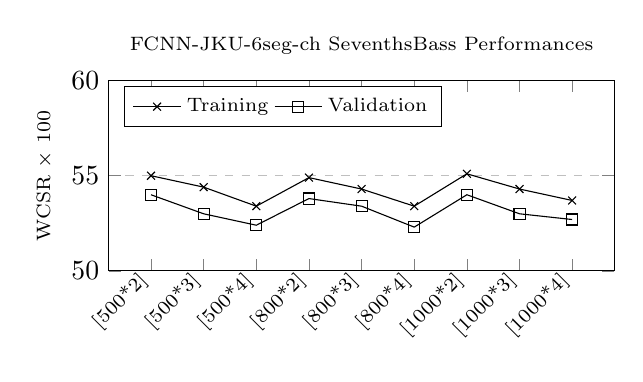
\begin{tikzpicture}
	\begin{axis}[
	title={FCNN-JKU-6seg-ch SeventhsBass Performances},
	title style = {font=\scriptsize},
	x label style={font=\scriptsize},
	symbolic x coords={[500*2],[500*3],[500*4],[800*2],[800*3],[800*4],[1000*2],[1000*3],[1000*4]},
	x tick label style={rotate=45,anchor=east, font=\scriptsize},
	xtick=data,
	ylabel={WCSR $\times$ 100},
	y label style={font=\scriptsize},
	ymin=50, ymax=60,
	ytick={50,55,60},
	legend pos=north west,
	legend style={legend columns=-1, font=\scriptsize},
	ymajorgrids=true,
	grid style=dashed,
	]
	
	\addplot[
	color=black,
	mark=x,
	]
	coordinates {
		([500*2],55.0)([500*3],54.4)([500*4],53.4)([800*2],54.9)([800*3],54.3)([800*4],53.4)([1000*2],55.1)([1000*3],54.3)([1000*4],53.7)
	};
	
	\addplot[
	color=black,
	mark=square,
	]
	coordinates {
		([500*2],54.0)([500*3],53.0)([500*4],52.4)([800*2],53.8)([800*3],53.4)([800*4],52.3)([1000*2],54.0)([1000*3],53.0)([1000*4],52.7)
	};
	\legend{Training, Validation} 
	\end{axis}
	\end{tikzpicture}
	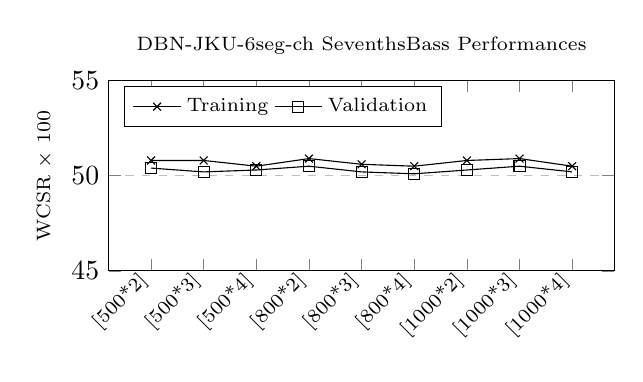
\begin{tikzpicture}
	\begin{axis}[
	title={DBN-JKU-6seg-ch SeventhsBass Performances},
	title style = {font=\scriptsize},
	x label style={font=\scriptsize},
	symbolic x coords={[500*2],[500*3],[500*4],[800*2],[800*3],[800*4],[1000*2],[1000*3],[1000*4]},
	x tick label style={rotate=45,anchor=east, font=\scriptsize},
	xtick=data,
	ylabel={WCSR $\times$ 100},
	y label style={font=\scriptsize},
	ymin=45, ymax=55,
	ytick={45,50,55},
	legend pos=north west,
	legend style={legend columns=-1, font=\scriptsize},
	ymajorgrids=true,
	grid style=dashed,
	]
	
	\addplot[
	color=black,
	mark=x,
	]
	coordinates {
		([500*2],50.8)([500*3],50.8)([500*4],50.5)([800*2],50.9)([800*3],50.6)([800*4],50.5)([1000*2],50.8)([1000*3],50.9)([1000*4],50.5)
	};
	
	\addplot[
	color=black,
	mark=square,
	]
	coordinates {
		([500*2],50.4)([500*3],50.2)([500*4],50.3)([800*2],50.5)([800*3],50.2)([800*4],50.1)([1000*2],50.3)([1000*3],50.5)([1000*4],50.2)
	};
	\legend{Training, Validation} 
	\end{axis}
	\end{tikzpicture}
	\caption{Exploring different network configurations at -ch level. All models are trained with JKU-6seg-ch.}
	\label{fig:dbn-ch-configs}
\end{figure}

\Hsection{-ns level}
Figure~\ref{fig:dbn-ns-configs} shows the scores of a set of 6seg-ns models with different neural nets and network configurations. In the case of FCNN, different from the ones shown in the Figure~\ref{fig:dbn-ch-configs}, the validation scores are all focused around 50. As for DBN, there is a trend of performance downgrade along both network width and depth dimensions. In both cases the variances between training and validation scores are very small.
\pgfplotsset{width=8cm,height=4cm,every node near coord/.append style={font=\scriptsize}}
\begin{figure}[htb]
	\centering
	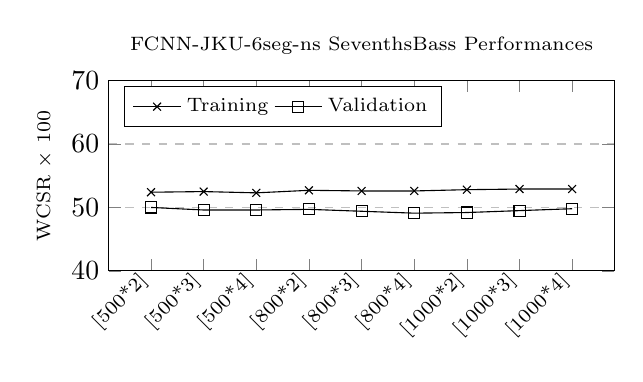
\begin{tikzpicture}
	\begin{axis}[
	title={FCNN-JKU-6seg-ns SeventhsBass Performances},
	title style = {font=\scriptsize},
	x label style={font=\scriptsize},
	symbolic x coords={[500*2],[500*3],[500*4],[800*2],[800*3],[800*4],[1000*2],[1000*3],[1000*4]},
	x tick label style={rotate=45,anchor=east, font=\scriptsize},
	xtick=data,
	ylabel={WCSR $\times$ 100},
	y label style={font=\scriptsize},
	ymin=40, ymax=70,
	ytick={40,50,60,70},
	legend pos=north west,
	legend style={legend columns=-1, font=\scriptsize},
	ymajorgrids=true,
	grid style=dashed,
	]
	\addplot[
	color=black,
	mark=x,
	]
	coordinates {
		([500*2],52.4)([500*3],52.5)([500*4],52.3)([800*2],52.7)([800*3],52.6)([800*4],52.6)([1000*2],52.8)([1000*3],52.9)([1000*4],52.9)
	};
	
	\addplot[
	color=black,
	mark=square,
	]
	coordinates {
		([500*2],50.0)([500*3],49.6)([500*4],49.6)([800*2],49.7)([800*3],49.4)([800*4],49.1)([1000*2],49.2)([1000*3],49.5)([1000*4],49.8)
	};
	\legend{Training, Validation} 
	\end{axis}
	\end{tikzpicture}
	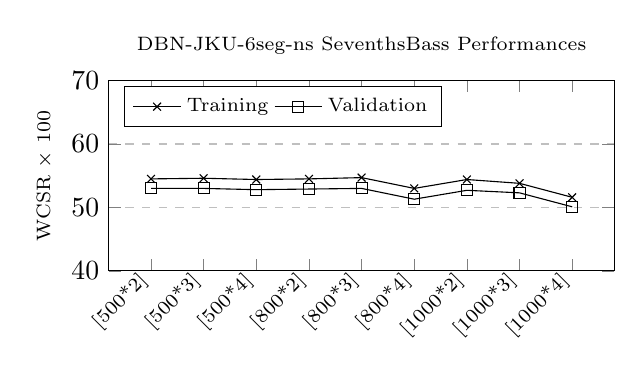
\begin{tikzpicture}
	\begin{axis}[
	title={DBN-JKU-6seg-ns SeventhsBass Performances},
	title style = {font=\scriptsize},
	x label style={font=\scriptsize},
	symbolic x coords={[500*2],[500*3],[500*4],[800*2],[800*3],[800*4],[1000*2],[1000*3],[1000*4]},
	x tick label style={rotate=45,anchor=east, font=\scriptsize},
	xtick=data,
	ylabel={WCSR $\times$ 100},
	y label style={font=\scriptsize},
	ymin=40, ymax=70,
	ytick={40,50,60,70},
	legend pos=north west,
	legend style={legend columns=-1, font=\scriptsize},
	ymajorgrids=true,
	grid style=dashed,
	]
	\addplot[
	color=black,
	mark=x,
	]
	coordinates {
		([500*2],54.5)([500*3],54.6)([500*4],54.4)([800*2],54.5)([800*3],54.7)([800*4],53.0)([1000*2],54.4)([1000*3],53.8)([1000*4],51.6)
	};
	
	\addplot[
	color=black,
	mark=square,
	]
	coordinates {
		([500*2],53.0)([500*3],53.0)([500*4],52.8)([800*2],52.9)([800*3],53.0)([800*4],51.3)([1000*2],52.7)([1000*3],52.3)([1000*4],50.1)
	};
	\legend{Training, Validation} 
	\end{axis}
	\end{tikzpicture}
	\caption{Exploring different network configurations at -ns level. All models are trained with JKU-6seg-ns.}
	\label{fig:dbn-ns-configs}
\end{figure}

\Hsection{remarks}
There is an implicit message in Figures~\ref{fig:dbn-ch-configs} and ~\ref{fig:dbn-ns-configs} that all FCNN-ch models outperform FCNN-ns models. This is largely due to the feature prior imposed by the bass-treble chromagram, which is specifically handcrafted for chord recognition. That means the model with this feature as input has already been informed some prior knowledge about the chord recognition problem. While notegram is a less biased feature output from a much earlier feature extraction stage.

This observation could be used to explain why FCNN-ch models perform worse as their networks grow deeper, as every extra layer between input and output will tend to weaken the prior at the input. At the same time these layers will learn some other regularities. The results here show that unfortunately the deeper networks are unable to learn more useful regularities than the prior information already conveyed in the bass-treble chromagram.

The FCNN-ns models are unable to outperform FCNN-ch models. It is clear from the low variances of FCNN-ns that the models have already saturated their learning powers. But at the same time they all suffer from high bias. This indicates a number of possibilities: a learning framework with inadequate modeling power, or underrepresented data (insufficiency, imbalanced, or inconsistency), or both of them.

Finally, the performance drop of wider and deeper DBN-ns models is believed to be caused by the vanishing gradients, since the proposed implementation of DBN uses sigmoid activation functions.

\subsection{Segment tiling} \label{sec:3-p3}

\Hsection{-ch level}
This subsection explores the effect of segment tiling ($N$seg) at -ch level. A set of models are implemented using JKU-ch-[800*2] with different segment tiling schemes and neural nets. [800*2] in BLSTM-RNN means there are one forward and one backward hidden layer, each having 800 LSTM units.

As shown in Figure~\ref{fig:N-frame}: FCNN is hardly affected by $N$seg; DBN tends to score better with larger $N$; BLSTM-RNN grows gently when $N$ is less than 3, and stays steady afterwards. All models in this set have very small training-validation variances.
\pgfplotsset{width=8cm,height=4cm,every node near coord/.append style={font=\scriptsize}}
\begin{figure}[htb]
	\centering
	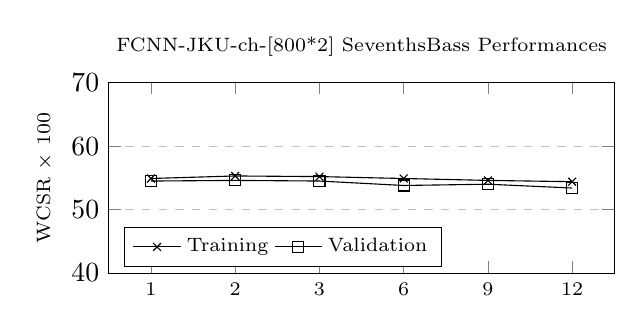
\begin{tikzpicture}
	\begin{axis}[
	title={FCNN-JKU-ch-[800*2] SeventhsBass Performances},
	title style = {font=\scriptsize},
	x label style={font=\scriptsize},
	symbolic x coords={1,2,3,6,9,12},
	x tick label style={font=\scriptsize},
	xtick=data,
	ylabel={WCSR $\times$ 100},
	y label style={font=\scriptsize},
	ymin=40, ymax=70,
	ytick={40,50,60,70},
	legend pos=south west,
	legend style={legend columns=-1, font=\scriptsize},
	ymajorgrids=true,
	grid style=dashed,
	]
	\addplot[ % Training
	color=black,
	mark=x,
	]
	coordinates {
		(1,54.9)(2,55.3)(3,55.2)(6,54.9)(9,54.6)(12,54.4)
	};
	
	\addplot[ % validation
	color=black,
	mark=square,
	]
	coordinates {
		(1,54.5)(2,54.6)(3,54.5)(6,53.8)(9,54.0)(12,53.4)
	};
	\legend{Training, Validation} 
	\end{axis}
	\end{tikzpicture}
	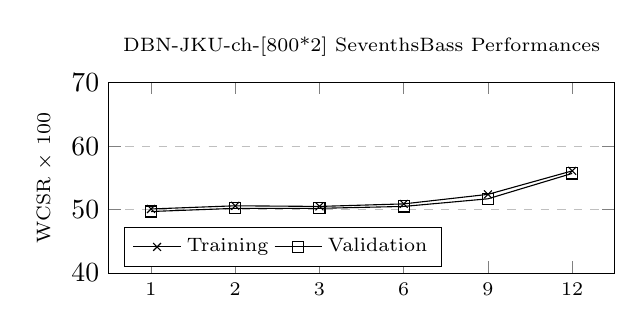
\begin{tikzpicture}
	\begin{axis}[
	title={DBN-JKU-ch-[800*2] SeventhsBass Performances},
	title style = {font=\scriptsize},
	x label style={font=\scriptsize},
	symbolic x coords={1,2,3,6,9,12},
	x tick label style={font=\scriptsize},
	xtick=data,
	ylabel={WCSR $\times$ 100},
	y label style={font=\scriptsize},
	ymin=40, ymax=70,
	ytick={40,50,60,70},
	legend pos=south west,
	legend style={legend columns=-1, font=\scriptsize},
	ymajorgrids=true,
	grid style=dashed,
	]
	\addplot[ % Training
	color=black,
	mark=x,
	]
	coordinates {
		(1,50.1)(2,50.6)(3,50.5)(6,50.9)(9,52.4)(12,56.1)
	};
	
	\addplot[ % validation
	color=black,
	mark=square,
	]
	coordinates {
		(1,49.7)(2,50.2)(3,50.2)(6,50.5)(9,51.7)(12,55.7)
	};
	\legend{Training, Validation} 
	\end{axis}
	\end{tikzpicture}
	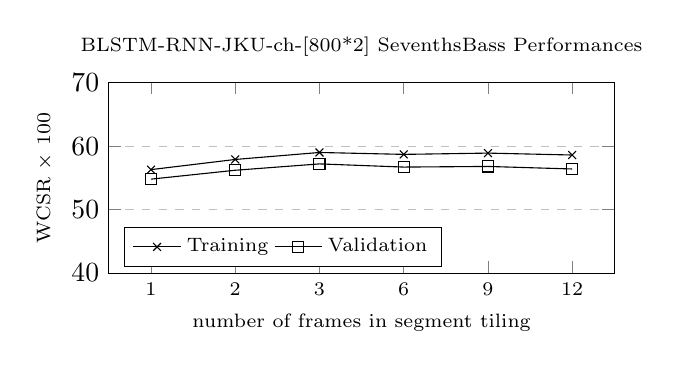
\begin{tikzpicture}
	\begin{axis}[
	title={BLSTM-RNN-JKU-ch-[800*2] SeventhsBass Performances},
	title style = {font=\scriptsize},
	x label style={font=\scriptsize},
	symbolic x coords={1,2,3,6,9,12},
	x tick label style={font=\scriptsize},
	xtick=data,
	xlabel={number of frames in segment tiling},
	ylabel={WCSR $\times$ 100},
	y label style={font=\scriptsize},
	ymin=40, ymax=70,
	ytick={40,50,60,70},
	legend pos=south west,
	legend style={legend columns=-1, font=\scriptsize},
	ymajorgrids=true,
	grid style=dashed,
	]
	\addplot[ % Training
	color=black,
	mark=x,
	]
	coordinates {
		(1,56.3)(2,57.9)(3,59.0)(6,58.7)(9,58.9)(12,58.6)
	};
	
	\addplot[ % validation
	color=black,
	mark=square,
	]
	coordinates {
		(1,54.8)(2,56.2)(3,57.2)(6,56.7)(9,56.8)(12,56.4)
	};
	\legend{Training, Validation} 
	\end{axis}
	\end{tikzpicture}
	\caption{Exploring effect of segment tiling at -ch level. All models are trained with JKU-ch-[800*2]}
	\label{fig:N-frame}
\end{figure}

\Hsection{-ns level}
A set of models are implemented using JKU-ns-[800*2] with different segment tiling schemes and neural nets. The experiment results are shown in Figure~\ref{fig:N-frame-ns}. All models are quite unaffected by $N$seg, particularly when $N$ is greater than 2. Different from those at -ch level, the variances of these models are larger, especially the BLSTM-RNN models.

\pgfplotsset{width=8cm,height=4cm,every node near coord/.append style={font=\scriptsize}}
\begin{figure}[htb]
	\centering
	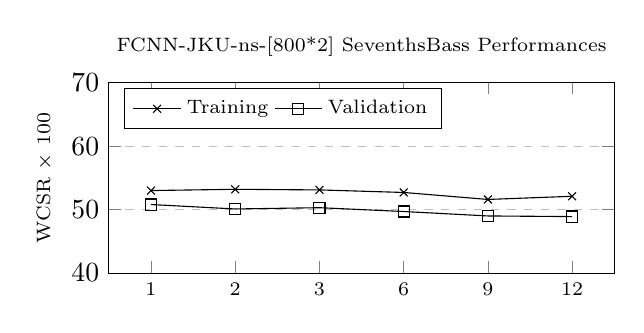
\begin{tikzpicture}
	\begin{axis}[
	title={FCNN-JKU-ns-[800*2] SeventhsBass Performances},
	title style = {font=\scriptsize},
	x label style={font=\scriptsize},
	symbolic x coords={1,2,3,6,9,12},
	x tick label style={font=\scriptsize},
	xtick=data,
	ylabel={WCSR $\times$ 100},
	y label style={font=\scriptsize},
	ymin=40, ymax=70,
	ytick={40,50,60,70},
	legend pos=north west,
	legend style={legend columns=-1, font=\scriptsize},
	ymajorgrids=true,
	grid style=dashed,
	]
	\addplot[ % Training
	color=black,
	mark=x,
	]
	coordinates {
		(1,53.0)(2,53.2)(3,53.1)(6,52.7)(9,51.6)(12,52.1)
	};
	
	\addplot[ % validation
	color=black,
	mark=square,
	]
	coordinates {
		(1,50.8)(2,50.1)(3,50.3)(6,49.7)(9,49.0)(12,48.9)
	};
	\legend{Training, Validation} 
	\end{axis}
	\end{tikzpicture}
	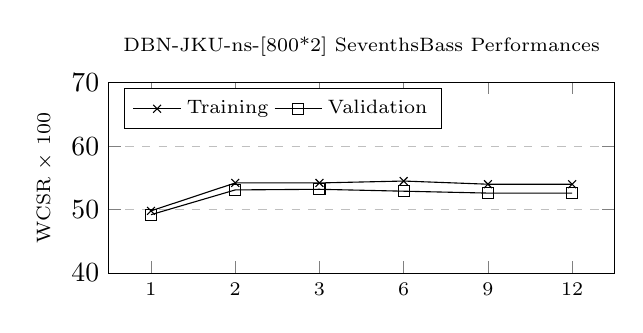
\begin{tikzpicture}
	\begin{axis}[
	title={DBN-JKU-ns-[800*2] SeventhsBass Performances},
	title style = {font=\scriptsize},
	x label style={font=\scriptsize},
	symbolic x coords={1,2,3,6,9,12},
	x tick label style={font=\scriptsize},
	xtick=data,
	ylabel={WCSR $\times$ 100},
	y label style={font=\scriptsize},
	ymin=40, ymax=70,
	ytick={40,50,60,70},
	legend pos=north west,
	legend style={legend columns=-1, font=\scriptsize},
	ymajorgrids=true,
	grid style=dashed,
	]
	\addplot[ % Training
	color=black,
	mark=x,
	]
	coordinates {
		(1,49.8)(2,54.2)(3,54.2)(6,54.5)(9,54.0)(12,54.0)
	};
	
	\addplot[ % validation
	color=black,
	mark=square,
	]
	coordinates {
		(1,49.2)(2,53.1)(3,53.2)(6,52.9)(9,52.6)(12,52.6)
	};
	\legend{Training, Validation} 
	\end{axis}
	\end{tikzpicture}
	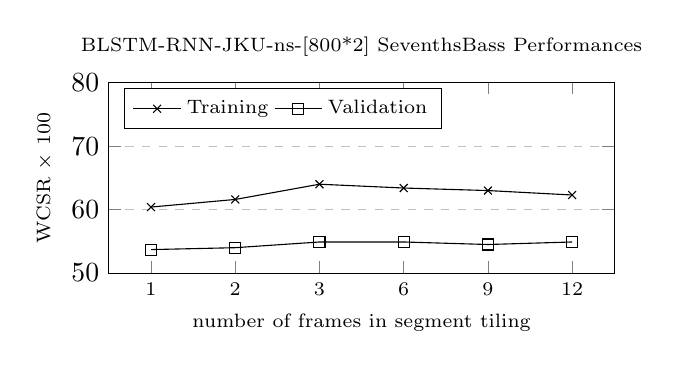
\begin{tikzpicture}
	\begin{axis}[
	title={BLSTM-RNN-JKU-ns-[800*2] SeventhsBass Performances},
	title style = {font=\scriptsize},
	x label style={font=\scriptsize},
	symbolic x coords={1,2,3,6,9,12},
	x tick label style={font=\scriptsize},
	xtick=data,
	xlabel={number of frames in segment tiling},
	ylabel={WCSR $\times$ 100},
	y label style={font=\scriptsize},
	ymin=50, ymax=80,
	ytick={50,60,70,80},
	legend pos=north west,
	legend style={legend columns=-1, font=\scriptsize},
	ymajorgrids=true,
	grid style=dashed,
	]
	\addplot[ % Training
	color=black,
	mark=x,
	]
	coordinates {
		(1,60.4)(2,61.6)(3,64.0)(6,63.4)(9,63.0)(12,62.3)
	};
	
	\addplot[ % validation
	color=black,
	mark=square,
	]
	coordinates {
		(1,53.7)(2,54.0)(3,54.9)(6,54.9)(9,54.5)(12,54.9)
	};
	\legend{Training, Validation} 
	\end{axis}
	\end{tikzpicture}
	\caption{Exploring effect of segment tiling at -ns level. All models are trained with JKU-ns-[800*2]}
	\label{fig:N-frame-ns}
\end{figure}

\Hsection{remarks}
A model becomes more complex with a larger $N$seg. As the model becomes more complex, one could expect either less bias, or more variance. One could observe slight decreases of biases from $N$=1 to 3 in models of DBN-ch, BLSTM-RNN-ch, DBN-ns and BLSTM-RNN-ns, but there is no obvious change beyond $N$=3 except for DBN-ch. The FCNN models are all quite unaffected by $N$seg.

Except for BLSTM-RNN-ns, all other models have large biases and low variances, which indicates that these models are indeed unsuitable for the underlying data, or the data itself contains a lot of noise. The BLSTM-RNN-ns models have much lower biases than the others, and yet they have much larger variances, which indicates that there is extra room for improvement in terms of their generalization ability.

\subsection{Training data size}\label{sec:3-p5}

\Hsection{-ch level}
Figure~\ref{fig:ch-data} shows the performances of different 6seg-ch-[800*2] models with different neural nets as a function of dataset sizes. In all three plots, there are clear trends that the increments of training data size reduce the models' biases, though the trends are slightly reversed from JKUR to JKURB. While the variances of FCNN's and DBN's models remain being small, the variances of BLSTM-RNN models decrease with the increment of training data, as one would normally expect.
\begin{figure}[htb]
	\centering
	\pgfplotsset{width=8cm,height=4cm,every node near coord/.append style={font=\scriptsize}}
	\subfigure{
		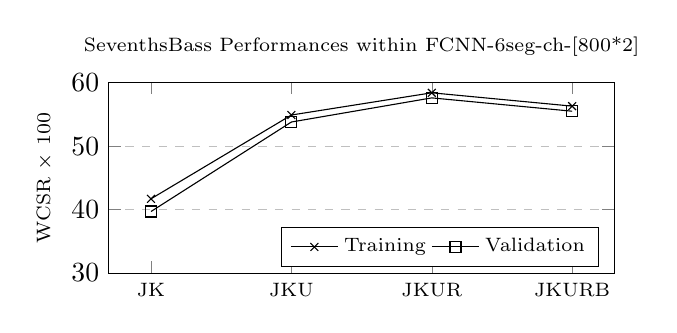
\begin{tikzpicture}
		\begin{axis}[
		title={SeventhsBass Performances within FCNN-6seg-ch-[800*2]},
		title style = {font=\scriptsize},
		x label style={font=\scriptsize},
		symbolic x coords={JK,JKU,JKUR,JKURB},
		x tick label style={font=\scriptsize},
		xtick=data,
		ylabel={WCSR $\times$ 100},
		y label style={font=\scriptsize},
		ymin=30, ymax=60,
		ytick={30,40,50,60},
		legend pos=south east,
		legend style={legend columns=-1, font=\scriptsize},
		ymajorgrids=true,
		grid style=dashed,
		]
		\addplot[ % Training
		color=black,
		mark=x,
		]
		coordinates {(JK,41.7)(JKU,54.9)(JKUR,58.4)(JKURB,56.3)};
		
		\addplot[ % validation
		color=black,
		mark=square,
		]
		coordinates {(JK,39.7)(JKU,53.8)(JKUR,57.6)(JKURB,55.5)};
		\legend{Training, Validation} 
		\end{axis}
		\end{tikzpicture}
	}
	\subfigure{
		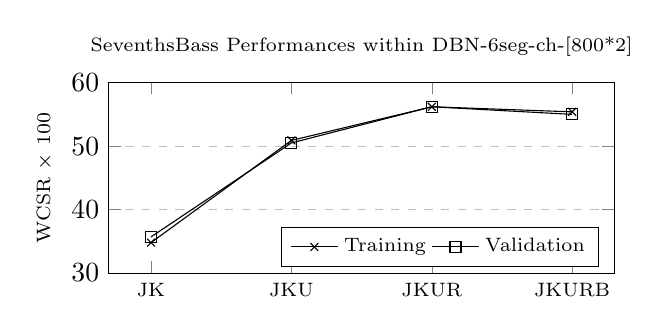
\begin{tikzpicture}
		\begin{axis}[
		title={SeventhsBass Performances within DBN-6seg-ch-[800*2]},
		title style = {font=\scriptsize},
		x label style={font=\scriptsize},
		symbolic x coords={JK,JKU,JKUR,JKURB},
		x tick label style={font=\scriptsize},
		xtick=data,
		ylabel={WCSR $\times$ 100},
		y label style={font=\scriptsize},
		ymin=30, ymax=60,
		ytick={30,40,50,60},
		legend pos=south east,
		legend style={legend columns=-1, font=\scriptsize},
		ymajorgrids=true,
		grid style=dashed,
		]
		\addplot[ % Training
		color=black,
		mark=x,
		]
		coordinates {(JK,34.8)(JKU,50.9)(JKUR,56.2)(JKURB,55.4)};
		
		\addplot[ % validation
		color=black,
		mark=square,
		]
		coordinates {(JK,35.7)(JKU,50.5)(JKUR,56.2)(JKURB,55.0)};
		\legend{Training, Validation} 
		\end{axis}
		\end{tikzpicture}
	}
	\subfigure{
		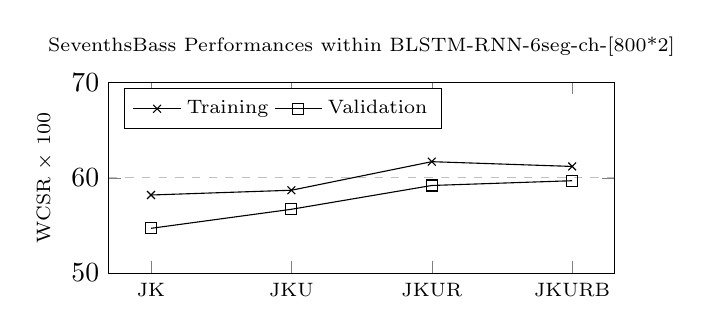
\begin{tikzpicture}
		\begin{axis}[
		title={SeventhsBass Performances within BLSTM-RNN-6seg-ch-[800*2]},
		title style = {font=\scriptsize},
		x label style={font=\scriptsize},
		symbolic x coords={JK,JKU,JKUR,JKURB},
		x tick label style={font=\scriptsize},
		xtick=data,
		ylabel={WCSR $\times$ 100},
		y label style={font=\scriptsize},
		ymin=50, ymax=70,
		ytick={50,60,70},
		legend pos=north west,
		legend style={legend columns=-1, font=\scriptsize},
		ymajorgrids=true,
		grid style=dashed,
		]
		\addplot[ % Training
		color=black,
		mark=x,
		]
		coordinates {(JK,58.2)(JKU,58.7)(JKUR,61.7)(JKURB,61.2)};
		
		\addplot[ % validation
		color=black,
		mark=square,
		]
		coordinates {(JK,54.7)(JKU,56.7)(JKUR,59.2)(JKURB,59.7)};
		\legend{Training, Validation} 
		\end{axis}
		\end{tikzpicture}
	}
	\caption{Exploring different training data size at -ch level. All models are trained with 6seg-ch-[800*2].}
	\label{fig:ch-data}
\end{figure}

\Hsection{-ns level}
Figure~\ref{fig:ns-data} shows the performances of different 6seg-ns-[800*2] models with different neural nets as a function of dataset sizes. These three set of models have similar behaviors as their -ch counterparts in Figure~\ref{fig:ch-data}. Interestingly for FCNN, the increment of data from JKUR to JKURB does not lead to a smaller variance (but much larger actually). The author currently has no clue why this might have happened, and thus consider this as an outlier. It might be caused by the noise introduced by dataset B, but the other two plots do not seem to support this reasoning.

\begin{figure}[htb]
	\centering
	\pgfplotsset{width=8cm,height=4cm,every node near coord/.append style={font=\scriptsize}}
	\subfigure{
		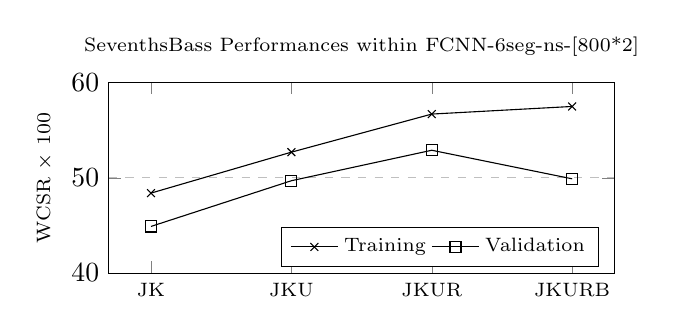
\begin{tikzpicture}
		\begin{axis}[
		title={SeventhsBass Performances within FCNN-6seg-ns-[800*2]},
		title style = {font=\scriptsize},
		%xlabel={Network Configuration},
		x label style={font=\scriptsize},
		symbolic x coords={JK,JKU,JKUR,JKURB},
		x tick label style={font=\scriptsize},
		xtick=data,
		ylabel={WCSR $\times$ 100},
		y label style={font=\scriptsize},
		ymin=40, ymax=60,
		ytick={40,50,60},
		legend pos=south east,
		legend style={legend columns=-1, font=\scriptsize},
		ymajorgrids=true,
		grid style=dashed,
		]
		\addplot[ % Training
		color=black,
		mark=x,
		]
		coordinates {(JK,48.4)(JKU,52.7)(JKUR,56.7)(JKURB,57.5)};
		
		\addplot[ % validation
		color=black,
		mark=square,
		]
		coordinates {(JK,44.9)(JKU,49.7)(JKUR,52.9)(JKURB,49.9)};
		\legend{Training, Validation} 
		\end{axis}
		\end{tikzpicture}
	}
	\subfigure{
		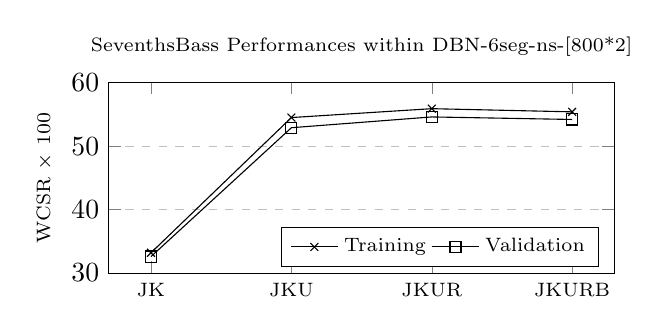
\begin{tikzpicture}
		\begin{axis}[
		title={SeventhsBass Performances within DBN-6seg-ns-[800*2]},
		title style = {font=\scriptsize},
		%xlabel={Network Configuration},
		x label style={font=\scriptsize},
		symbolic x coords={JK,JKU,JKUR,JKURB},
		x tick label style={font=\scriptsize},
		xtick=data,
		ylabel={WCSR $\times$ 100},
		y label style={font=\scriptsize},
		ymin=30, ymax=60,
		ytick={30,40,50,60},
		legend pos=south east,
		legend style={legend columns=-1, font=\scriptsize},
		ymajorgrids=true,
		grid style=dashed,
		]
		\addplot[ % Training
		color=black,
		mark=x,
		]
		coordinates {(JK,33.2)(JKU,54.5)(JKUR,55.9)(JKURB,55.4)};
		
		\addplot[ % validation
		color=black,
		mark=square,
		]
		coordinates {(JK,32.6)(JKU,52.9)(JKUR,54.6)(JKURB,54.2)};
		\legend{Training, Validation} 
		\end{axis}
		\end{tikzpicture}
	}
	\subfigure{
		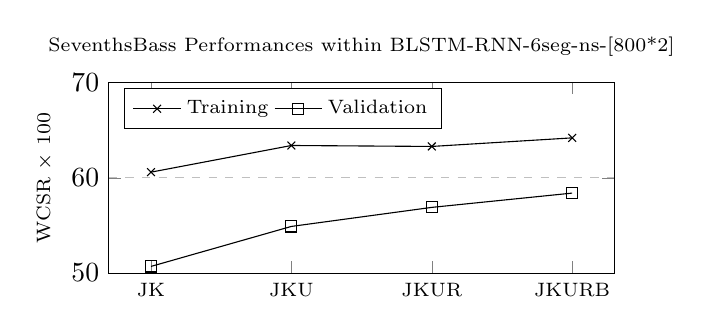
\begin{tikzpicture}
		\begin{axis}[
		title={SeventhsBass Performances within BLSTM-RNN-6seg-ns-[800*2]},
		title style = {font=\scriptsize},
		x label style={font=\scriptsize},
		symbolic x coords={JK,JKU,JKUR,JKURB},
		x tick label style={font=\scriptsize},
		xtick=data,
		ylabel={WCSR $\times$ 100},
		y label style={font=\scriptsize},
		ymin=50, ymax=70,
		ytick={50,60,70},
		legend pos=north west,
		legend style={legend columns=-1, font=\scriptsize},
		ymajorgrids=true,
		grid style=dashed,
		]
		\addplot[ % Training
		color=black,
		mark=x,
		]
		coordinates {(JK,60.6)(JKU,63.4)(JKUR,63.3)(JKURB,64.2)};
		
		\addplot[ % validation
		color=black,
		mark=square,
		]
		coordinates {(JK,50.7)(JKU,54.9)(JKUR,56.9)(JKURB,58.4)};
		\legend{Training, Validation} 
		\end{axis}
		\end{tikzpicture}
	}
	\caption{Exploring training data size at -ns level. All models are trained with 6seg-ns-[800*2].}
	\label{fig:ns-data}
\end{figure}

\Hsection{remarks}
Both Figure~\ref{fig:ch-data} and ~\ref{fig:ns-data} also show that in this group of experiments BLSTM-RNN-6seg-[800*2] models are having lower biases than FCNN's and DBN's (with the same other configurations).

In Figure~\ref{fig:ch-data}, at large data sizes (e.g. JKUR or JKURB) all three plots' validation scores are very close to each other, and the model' variances are small. It is difficult to tell which neural net has more advantage in representing the data at -ch level. In Figure~\ref{fig:ns-data}, on the contrary, although having larger variances, BLSTM-RNN-ns models are all scoring better than their FCNN and DBN counterparts in terms of validation scores. Since the variance decreases with the increase of training data size, one could expect a BLSTM-RNN-ns model to have an even lower variance when more data is available, which probably leads to a higher validation score.

Compared BLSTM-RNN-ch with BLSTM-RNN-ns at JKURB, one could notice that although the -ch model achieves a slightly better validation score, the -ns model could actually touch a potentially much lower bias. %It is difficult to judge which of them is better if more data is available.

\subsection{Skewed classes}\label{sec:3-p7}

A detail investigation of uncommon chords (chords that constitute the minor population) performances reveals the true potential of BLSTM-RNN that makes us believe it to be a better neural network at handling LVACE under the proposed framework. In short: 1) BLSTM-RNN performs much better than FCNN and DBN on uncommon chords as well as some common chords (chords that constitute the major population); 2) BLSTM-RNN scores much better in a balanced performance metric.
\begin{figure}[htb]
	\centering
    \includegraphics[width=1\columnwidth]{3/res/13-av_skewed.pdf}
	\caption{Comparison of common and uncommon chords in different neural nets. All models are trained with 6seg-[800*2].}
	\label{fig:blstm-long-tail}
\end{figure}

Figure~\ref{fig:blstm-long-tail} shows how different models perform on different chords (or ``chord types'', used interchangeably with ``chords'' in this context). These performances are reported as per chord \textit{WCSR}:
\begin{equation}
	\mathit{WCSR_{C} = {\sum{Length(C_i)*CSR_i} \over \sum{Length(C_i)}}},
	\label{eq:wcsrchord}
\end{equation}
where the subscript $i$ denotes the $i^{th}$ instance of the chord $C$ within the dataset. Among all chord types, \textit{maj}, \textit{min}, \textit{maj7}, \textit{min7} and \textit{7} are considered common chords, because they constitute the major population in pop/rock music \cite{burgoyne2011expert}. The other chords are considered as uncommon chords. As demonstrated in Figure~\ref{fig:blstm-long-tail}, the advantage of FCNN and DBN over BLSTM-RNN appears only in \textit{maj}, but BLSTM-RNN outperforms them by large amounts in most uncommon chords as well as other common chords.

\begin{figure}[htb]
	\centering
	\pgfplotsset{width=6cm,height=4cm,every node near coord/.append style={font=\scriptsize}}
	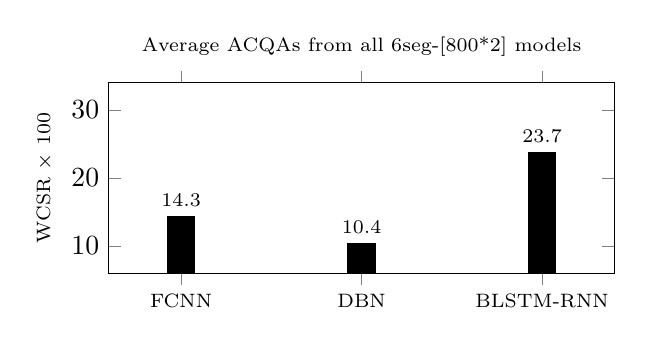
\begin{tikzpicture}
	\begin{axis}[
	title={Average ACQAs from all 6seg-[800*2] models},
	title style = {font=\scriptsize},
	ybar=8pt,
	enlargelimits=0.2,
	legend style={at={(0.5,-0.2)},
		anchor=north,legend columns=-1},
	ylabel={WCSR $\times$ 100},
	y label style={font=\scriptsize},
	symbolic x coords={FCNN,DBN,BLSTM-RNN},
	x tick label style={font=\scriptsize},
	xtick=data,
	ymin=10, ymax=30,
	nodes near coords,
	nodes near coords align={vertical},
	legend style={font=\scriptsize},
	]
	\addplot [ybar,fill=black,draw=black] coordinates {(FCNN,14.3)(DBN,10.4)(BLSTM-RNN,23.7)};
	\end{axis}
	\end{tikzpicture}
	\caption{Average ACQAs of \textit{SeventhsBass} Vocabulary. All models are trained with 6seg-[800*2].}
	\label{fig:acqa}
\end{figure}

To measure the well-roundedness of a model, ``Average Chord Quality Accuracy''(\textit{ACQA}) \cite{cho2014improved} is used. It is defined in Chapter~\ref{cp:background} Equation~\ref{eq:2-acqa} and recapped as follows
\begin{equation}
	\mathit{ACQA = {{\sum{WCSR_{C}}} \over {\#\,of\,chords}}}.
	\label{eq:3-acqa}
\end{equation}
Models that over-fit on a few chord types tend to get lower \textit{ACQA}s, while those well balanced ones will have higher \textit{ACQA}s. As shown in Figure~\ref{fig:acqa}, the average \textit{ACQA} of the BLSTM-RNN models outscores the average \textit{ACQA}s of the other two types of models by around 10 points. This well demonstrates that BLSTM-RNN models perform in a much more balanced way.

Here the author tries to provide a plausible explanation as to why BLSTM-RNN is a better neural network in solving LVACE problem than the other two. It is reasonable to think that BLSTM-RNN regards its input as a {\it sequence of frames}, while fully-connected networks (such as FCNN and DBN) regard their inputs as a \textit{flat vectors}. Therefore, while BLSTM-RNN tries to look for regularities within each pair of consecutive frames along the time direction, FCNN and DBN would search for regularities within every pair of consecutive or nonconsecutive frames as if they are not time related. In many chord recognition cases, the latter approach is more efficient when the input feature is already a good summarization of pitch class saliences (e.g. chromagram), but this approach overlooks the ``sequential order'' of frames, which results in the over-fitting of root position chords and under-fitting of inversion chords.

\subsection{Baseline Comparison} \label{sec:3-p9}

At last the proposed approach is compared with the baseline approach - Chordino. There is one representative for each deep neural net, all trained and cross-validated with JKURB-6seg-ns-[800*2]. They are compared with Chordino in terms of five categories: four \textit{WCSR}s and the \textit{ACQA} score.
\begin{figure}[htb]
	\centering
	\pgfplotsset{width=9cm,height=5cm,every node near coord/.append style={font=\tiny}}
	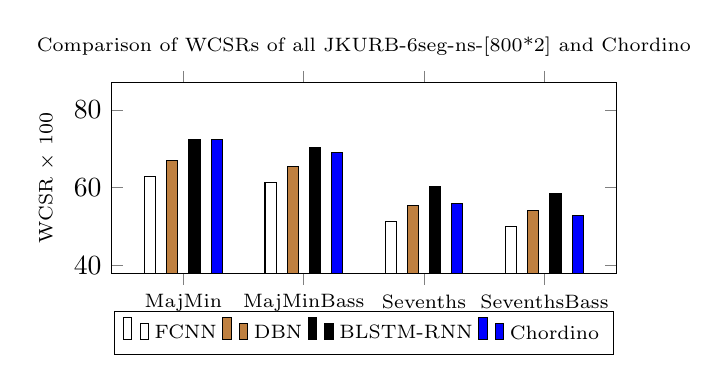
\begin{tikzpicture}
	\begin{axis}[
	title={Comparison of WCSRs of all JKURB-6seg-ns-[800*2] and Chordino},
	title style = {font=\scriptsize},
	ybar=4pt,
	bar width=4pt,
	enlargelimits=0.2,
	legend style={at={(0.5,-0.2)},
		anchor=north,legend columns=-1},
	ylabel={WCSR $\times$ 100},
	y label style={font=\scriptsize},
	symbolic x coords={MajMin,MajMinBass,Sevenths,SeventhsBass},
	x tick label style={font=\scriptsize},
	xtick=data,
	ymin=45, ymax=80,
	%nodes near coords,
	%nodes near coords align={vertical},
	legend style={font=\scriptsize},
	]
	\addplot [ybar,fill=white,draw=black] coordinates {(MajMin,62.9)(MajMinBass,61.2)(Sevenths,51.3)(SeventhsBass,49.9)};
	
	\addplot [ybar,fill=brown,draw=black] coordinates {(MajMin,67.0)(MajMinBass,65.5)(Sevenths,55.5)(SeventhsBass,54.2)};
	
	\addplot [ybar,fill=black,draw=black] coordinates {(MajMin,72.3)(MajMinBass,70.2)(Sevenths,60.2)(SeventhsBass,58.4)};
	
	\addplot [ybar,fill=blue,draw=black] coordinates {(MajMin,72.4)(MajMinBass,69.1)(Sevenths,55.8)(SeventhsBass,52.8)};
	
	\legend{FCNN, DBN, BLSTM-RNN, Chordino}
	\end{axis}
	\end{tikzpicture}
	\caption{Compare with Chordino. All models are trained with JKURB-6seg-ns-[800*2].}
	\label{fig:compchordino}
\end{figure}

\begin{figure}[htb]
	\centering
	\pgfplotsset{width=8cm,height=4cm,every node near coord/.append style={font=\scriptsize}}
	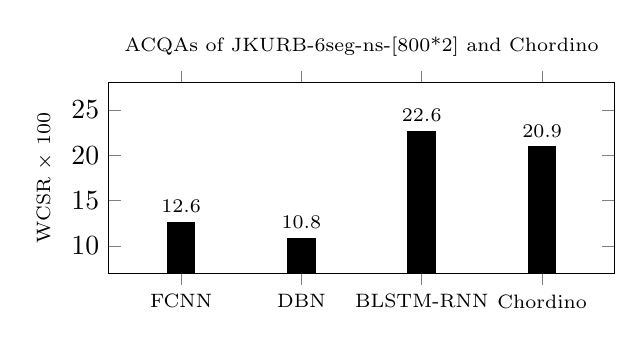
\begin{tikzpicture}
	\begin{axis}[
	title={ACQAs of JKURB-6seg-ns-[800*2] and Chordino},
	title style = {font=\scriptsize},
	ybar=8pt,
	enlargelimits=0.2,
	legend style={at={(0.5,-0.2)},
		anchor=north,legend columns=-1},
	ylabel={WCSR $\times$ 100},
	y label style={font=\scriptsize},
	symbolic x coords={FCNN,DBN,BLSTM-RNN,Chordino},
	x tick label style={font=\scriptsize},
	xtick=data,
	ymin=10, ymax=25,
	nodes near coords,
	nodes near coords align={vertical},
	legend style={font=\scriptsize},
	]
	\addplot [ybar,fill=black,draw=black] coordinates {(FCNN,12.6)(DBN,10.8)(BLSTM-RNN,22.6)(Chordino,20.9)};
	\end{axis}
	\end{tikzpicture}
	\caption{Comparison of ACQAs of JKURB-6seg-ns-[800*2] and Chordino}
	\label{fig:acqachordino}
\end{figure}

As shown in Figure~\ref{fig:compchordino}, the best representative BLSTM-RNN outperforms Chordino by a large amount in \textit{Sevenths} and \textit{SeventhsBass}, and it is fairly comparable with Chordino in \textit{MajMin} and \textit{MajMinBass}. The other two representatives are not scoring as good as Chordino in most categories.

In terms of versatility (Figure~\ref{fig:acqachordino}), Chordino is not bad at all, outperforming both FCNN's and DBN's representatives largely, but the most balanced system is still the BLSTM-RNN's representative.

\section{MIREX 2016 Results}
MIREX ACE 2016 features 4 sets of systems implemented by four different groups:
\begin{itemize}
\item CM1: Chordino, from Queen Mary University of London;
\item DK*: features three variants of the LVACE approach proposed in this chapter \cite{deng2016mirex} (note that DK4, which is from another design approach, is skipped in the following discussion);
\item FK*: implemented by Korzeniowski and Widmer, featuring the systems in two previous papers \cite{Korzeniowski2016feature,Korzeniowski2016convolutional}
\item KO1: shineChords, a time-frequency reassign approach proposed by Khadkevich and Omologo \cite{khadkevich2011time}.
\end{itemize}

\subsection{Dataset and Vocabulary}
It should be noted that except CM3, whose model parameters are all manually specified, all other systems involve extensive training:
\begin{itemize}
\item KO1's description does not mention its training set, but it is probably trained with the Isophonic dataset (MIREX 2009 set) \cite{burgoyne2014comparative}. This can be easily spot by simply noticing that, compared with other systems, it has too high a \textit{SeventhsBass} score in Isophonic, while not as high in other test sets.

\item FK* are trained with the Isophonic, Robbie Williams \footnote{\url{https://www.researchgate.net/publication/260399240\_Chord\_and\_Harmony\_annotations\_of\_the\_first\_five\_albums\_by\_Robbie\_Williams}}, RWC and the public part of McGill Billboard \footnote{\url{http://ddmal.music.mcgill.ca/billboard}} dataset.

\item DK* are trained with USPop and RWC dataset. Note that they do not contain any test set in MIREX ACE 2016. Note that DK1 is the DBN-6seg-ch-[800,800]-UR system and DK2 is the BLSTM-RNN-6seg-ch-[800,800]-UR system.
\end{itemize}

In terms of chord vocabulary, both DK3, FK* and KO1 only support \textit{majmin}, CM1 supports a large vocabulary including most types in \textit{SeventhsBass}, and DK1\&2 support exactly the \textit{SeventhsBass}.
\begin{table*}[h]
\centering
\scriptsize
\caption{MIREX 2016 Results}
\label{tab:3-mirex2016}
\begin{tabular}{|c|c|c|c|c|c|c|c|c|}\hline
Algorithm & R & Mm & MmB & S & SB & Seg & UnderSeg & OverSeg \\ \hline
Isophonics 2009\\ \hline
CM1 & 78.56 & 75.41 & 72.48 & 54.67 & 52.26 & 85.90 & 87.17 & 86.09\\ \hline
DK1 & 79.21 & 76.19 & 74.00 & 66.02 & 64.15 & 85.71 & 82.62 & 91.23\\ \hline
DK2 & 77.84 & 74.49 & 71.93 & 61.61 & 59.47 & 85.82 & 82.72 & 91.28\\ \hline
DK3 & 80.03 & 77.55 & 74.79 & 68.40 & 65.88 & 85.81 & 82.50 & 91.53\\ \hline
DK4 & 76.05 & 72.96 & 71.41 & 62.77 & 61.44 & 78.19 & 87.97 & 72.43\\ \hline
FK2 & 86.09 & 85.53 & 82.24 & 74.42 & 71.54 & 87.76 & 85.79 & 90.73\\ \hline
FK4 & 82.28 & 80.93 & 78.03 & 70.91 & 68.26 & 85.62 & 82.40 & 90.89\\ \hline
KO1 & 82.93 & 82.19 & 79.61 & 76.04 & 73.43 & 87.69 & 85.66 & 91.24\\ \hline
Billboard 2012 \\ \hline
CM1 & 74.15 & 72.22 & 70.21 & 55.35 & 53.40 & 83.64 & 85.31 & 83.39\\ \hline
DK1 & 75.28 & 73.57 & 71.87 & 59.98 & 58.53 & 83.35 & 80.26 & 88.52\\ \hline
DK2 & 73.77 & 71.69 & 69.86 & 58.66 & 57.00 & 83.57 & 80.40 & 88.70\\ \hline
DK3 & 75.92 & 74.75 & 72.69 & 53.42 & 51.67 & 83.39 & 79.97 & 88.92\\ \hline
DK4 & 72.59 & 70.85 & 69.78 & 56.29 & 55.36 & 76.13 & 87.72 & 70.05\\ \hline
FK2 & 85.64 & 85.38 & 82.55 & 60.70 & 58.38 & 87.62 & 86.09 & 90.13\\ \hline
FK4 & 79.23 & 78.62 & 76.20 & 56.53 & 54.51 & 85.09 & 81.98 & 89.94\\ \hline
KO1 & 77.45 & 75.58 & 73.51 & 57.68 & 55.82 & 84.16 & 82.80 & 87.44\\ \hline
Billboard 2013 \\ \hline
CM1 & 71.16 & 67.28 & 65.20 & 48.99 & 47.17 & 81.54 & 83.11 & 82.63\\ \hline
DK1 & 72.06 & 68.69 & 67.26 & 54.54 & 53.29 & 80.82 & 77.58 & 88.06\\ \hline
DK2 & 70.18 & 66.54 & 64.66 & 52.97 & 51.41 & 80.85 & 77.68 & 88.02\\ \hline
DK3 & 72.39 & 68.53 & 66.55 & 48.99 & 47.28 & 80.76 & 77.26 & 88.30\\ \hline
DK4 & 69.56 & 65.83 & 64.78 & 51.81 & 50.93 & 74.55 & 86.31 & 69.18\\ \hline
FK2 & 80.07 & 77.89 & 75.42 & 55.41 & 53.22 & 82.94 & 82.43 & 86.80\\ \hline
FK4 & 74.66 & 71.85 & 69.44 & 51.93 & 49.80 & 80.61 & 77.19 & 88.70\\ \hline
KO1 & 75.36 & 71.39 & 69.43 & 53.57 & 51.78 & 81.63 & 79.61 & 87.75\\ \hline
JayChou 2015 \\ \hline
CM1 & 72.75 & 72.08 & 65.48 & 54.39 & 48.98 & 86.60 & 86.89 & 86.91\\ \hline
DK1 & 74.70 & 73.87 & 70.33 & 54.98 & 52.25 & 86.76 & 82.78 & 91.79\\ \hline
DK2 & 72.19 & 72.55 & 69.10 & 54.09 & 51.46 & 87.09 & 83.35 & 91.75\\ \hline
DK3 & 75.01 & 74.75 & 63.56 & 49.27 & 40.24 & 86.76 & 82.54 & 92.08\\ \hline
DK4 & 71.51 & 69.03 & 65.93 & 50.07 & 47.45 & 78.11 & 87.87 & 70.56\\ \hline
FK2 & 79.51 & 78.66 & 68.15 & 50.69 & 42.34 & 86.81 & 85.43 & 88.56\\ \hline
FK4 & 76.13 & 75.44 & 64.36 & 49.69 & 40.74 & 84.55 & 81.22 & 88.95\\ \hline
KO1 & 78.73 & 77.69 & 66.87 & 54.16 & 44.55 & 88.46 & 87.12 & 90.11\\ \hline
RobbieWilliams 2016 \\ \hline
CM1 & 81.90 & 78.25 & 76.05 & 57.92 & 55.90 & 87.96 & 88.96 & 87.45\\ \hline
DK1 & 81.50 & 77.77 & 76.10 & 68.88 & 67.34 & 87.03 & 83.22 & 92.11\\ \hline
DK2 & 79.01 & 75.97 & 73.57 & 65.26 & 62.98 & 87.20 & 83.40 & 92.23\\ \hline
DK3 & 81.85 & 78.56 & 76.16 & 74.71 & 72.55 & 86.98 & 82.95 & 92.34\\ \hline
DK4 & 78.92 & 75.15 & 73.66 & 66.72 & 65.34 & 81.82 & 88.44 & 76.88\\ \hline
FK2 & 88.53 & 87.23 & 84.19 & 82.57 & 79.88 & 90.04 & 88.62 & 91.88\\ \hline
FK4 & 83.37 & 80.96 & 78.42 & 77.04 & 74.76 & 87.22 & 84.50 & 91.02\\ \hline
KO1 & 83.55 & 80.33 & 78.16 & 73.54 & 71.39 & 88.04 & 85.39 & 91.68\\ \hline
\end{tabular}
\end{table*}


\subsection{Results and Discussions}
Table~\ref{tab:3-mirex2016} shows the results of MIREX ACE 2016 (for brevity in the tables, B = \textit{Bass}, Mm = \textit{MajMin}, MmB = \textit{MajMinBass}, R = \textit{Root}, S = \textit{Sevenths}, SB = \textit{SeventhsBass}, Seg = \textit{Segmentation Quality}). Within the large vocabulary context of this thesis, the main focus of the results is the \textit{SeventhsBass} column.

In Isophonic test, KO1 gets the highest score. But this is probably because of its over-fitting the data, as explained previously, that it actually scores much lower in tests that it does not previously know, such as JayChou 2015. Both FK2 and FK4 come next to KO1, but unfortunately they are all informed with this test set. Since it is not clear to what extend the systems over-learn the data, the results of this test is not statistically valid to deduce any reasonable conclusions regarding these systems.

In Billboard 2012 and 2013 tests, the best performances are both from DK1. Although FK* learn from part of the test set, they somehow does not outperform DK1. Moreover, DK1 outscore KO1 by about 3 points in both tests, which demonstrates a better generalization capability in DK1 system.

JayChou 2015 test is probably the most convincing one, since none of the systems are learning this set, and on the other hand it has more than 20\% of chords other than \textit{maj}, \textit{min} and \textit{sevenths}, which is much more than those in other test sets. The performance on this test could well demonstrate the system's vocabulary versatility. This can be noticed by making comparison within the DK* systems, where DK1 and DK2 perform much better than DK3 in \textit{SeventhsBass}. The best two systems in this test are DK1 and DK2, outscoring the FK* systems by around 10 points, and the KO1 system by about 8 points.

Robbie Williams test somehow shows the reverse ranking of JayChou 2015. DK3 leads both DK1 and DK2 by about 5 and 10 points. FK* are the best performing ones, but unfortunately they might over-learn the data. It is interesting to note that KO1 scores 71.39, slightly less that DK3's 72.55. This strongly indicates that this test is mainly composed of \textit{maj}, \textit{min} and \textit{sevenths} (probably > 90\%), which is very similar to the chord composition of the Isophonic set. Therefore systems that only support a small chord vocabulary will have a huge advantage by not being able to have confusions on long-tail chords.

\section{On Smaller Vocabularies}
This chapter is mainly developed based on large vocabulary, specifically, the \textit{SeventhsBass} vocabulary. In order to do a comparison between the proposed system framework and other approaches, a set of experiments are conducted using two smaller vocabularies: 1, \textit{MajMin}; 2, \textit{Full121} vocabulary introduced by Mauch \cite{mauch2010automatic} (also mentioned in Section~\ref{sec:2-largevocab}). For \textit{MajMin} system implementation, each label in the training set will be mapped to its \textit{MajMin} form following a normal chord mapping scheme \cite{harte2010towards,pauwels2013evaluating}. As a result, each deep learning model will be trained on a dataset with only \textit{MajMin} labels. For \textit{Full121} implementation, a slightly modified version of chord mapping strategy \cite{mauch2010automatic} is followed.

\subsection{On MajMin}
Table~\ref{tab:3-overallres} shows a \textit{SeventhsBass} evaluation comparison, where all systems, except for Chordino, only supports \textit{MajMin} vocabulary. The results show that on one hand the overall performances of these systems are only fairly comparable with those in Section~\ref{sec:3-p9}, on the other hand the \textit{ACQA} of these systems are all much lower because of a much smaller vocabulary than Chordino's.
\begin{table}[h]
\footnotesize
\centering
\caption{Overall WCSR scores; All systems, besides Chordino, are trained with CJKUR-[800*2], tested on the TheBeatles180 dataset, with only MajMin vocabulary support.}
\label{tab:3-overallres}
\begin{tabular}{|c|c|c|c|c|c|c|c|c|}\hline
System & B & Mm & MmB & R & S & SB & Seg & ACQA \\ \hline
Chordino & 76.41 & 74.30 & 71.40 & 77.19 & 52.99 & 50.60 & 83.87 & 16.61\\ \hline
FCNN-ch & 74.71 & 73.25 & 71.22 & 75.74 & 65.08 & 63.18 & 83.57 & 8.42\\ \hline
DBN-ch & 77.04 & 75.50 & 73.39 & 78.10 & 67.26 & 65.30 & 83.78 & 8.71\\ \hline
BLSTM-RNN-ch & 76.88 & 75.05 & 72.84 & 78.11 & 66.58 & 64.50 & 83.74 & 8.75\\ \hline
FCNN-ns & 72.65 & 70.00 & 68.14 & 73.35 & 62.72 & 60.98 & 83.59 & 7.81\\ \hline
DBN-ns & 72.91 & 70.96 & 69.14 & 73.66 & 63.33 & 61.66 & 83.44 & 8.05\\ \hline
BLSTM-RNN-ns & 76.04 & 73.98 & 71.99 & 76.85 & 65.85 & 64.03 & 83.76 & 8.54\\ \hline
\end{tabular}
\end{table}

Table~\ref{tab:3-detailres} shows the \textit{SeventhsBass} categorical breakdown. Take DBN-ch as a representative, since it only supports \textit{MajMin}, its $maj$ and $min$ scores are much higher than the Chordino's. As the two chord types comprise of the majority of the dataset's population, that's why it has a much higher \textit{SeventhsBass} score in Table~\ref{tab:3-overallres}. However, by relaxing the evaluation strength from \textit{SeventhsBass} to \textit{Sevenths} and to \textit{MajMin}, the performance difference between DBN-ch and Chordino becomes less and less.

\begin{landscape}
\thispagestyle{plain}
\begin{table*}[h]
\scriptsize
\caption{Detail SeventhsBass WCSR scores. All systems, besides Chordino, are trained with CJKUR-[800*2], with only MajMin vocabulary support. M = major, m = minor, N = N.C (no chord). The \%B row shows the composition of chords in the test set.}
\label{tab:3-detailres}
\begin{tabular}{|c|c|c|c|c|c|c|c|c|c|c|c|c|c|c|c|c|c|c|c|}\hline
\%B & 2.01 & 0.95 & 63.31 & 0.02 & 0.17 & 0.27 & 0.82 & 0.08 & 0.06 & 0.39 & 8.33 & 0.61 & 0.44 & 14.99 & 0.01 & 0.06 & 0.41 & 2.37 & 4.63\\ \hline
 & M/5 & M/3 & M & M7/5 & M7/3 & M7/7 & M7 & 7/5 & 7/3 & 7/b7 & 7 & m/5 & m/b3 & m & m7/5 & m7/b3 & m7/b7 & m7 & N\\ \hline
Chordino & 19.9 & 17.1 & 54.4 & 0.0 & 0.0 & 0.0 & 55.6 & 0.0 & 0.0 & 5.7 & 41.0 & 0.0 & 0.0 & 54.3 & 0.0 & 0.0 & 0.0 & 51.0 & 2.2\\ \hline
FCNN-ch & 0.0 & 0.0 & 77.6 & 0.0 & 0.0 & 0.0 & 0.0 & 0.0 & 0.0 & 0.0 & 0.0 & 0.0 & 0.0 & 74.0 & 0.0 & 0.0 & 0.0 & 0.0 & 2.8\\ \hline
DBN-ch & 0.0 & 0.0 & 80.0 & 0.0 & 0.0 & 0.0 & 0.0 & 0.0 & 0.0 & 0.0 & 0.0 & 0.0 & 0.0 & 76.8 & 0.0 & 0.0 & 0.0 & 0.0 & 3.0\\ \hline
BLSTM-RNN-ch & 0.0 & 0.0 & 79.3 & 0.0 & 0.0 & 0.0 & 0.0 & 0.0 & 0.0 & 0.0 & 0.0 & 0.0 & 0.0 & 78.2 & 0.0 & 0.0 & 0.0 & 0.0 & 2.5\\ \hline
FCNN-ns & 0.0 & 0.0 & 76.4 & 0.0 & 0.0 & 0.0 & 0.0 & 0.0 & 0.0 & 0.0 & 0.0 & 0.0 & 0.0 & 64.2 & 0.0 & 0.0 & 0.0 & 0.0 & 2.9\\ \hline
DBN-ns & 0.0 & 0.0 & 76.3 & 0.0 & 0.0 & 0.0 & 0.0 & 0.0 & 0.0 & 0.0 & 0.0 & 0.0 & 0.0 & 68.6 & 0.0 & 0.0 & 0.0 & 0.0 & 2.9\\ \hline
BLSTM-RNN-ns & 0.0 & 0.0 & 79.0 & 0.0 & 0.0 & 0.0 & 0.0 & 0.0 & 0.0 & 0.0 & 0.0 & 0.0 & 0.0 & 74.7 & 0.0 & 0.0 & 0.0 & 0.0 & 2.7\\ \hline
\end{tabular}
\end{table*}
\end{landscape}

\subsection{On Full121}
Table~\ref{tab:3-full} shows the WCSR results of \textit{Full121} vocabulary with the same test set. Table~\ref{tab:3-fullhp} and ~\ref{tab:3-fullmbk} shows the \textit{Full121} scores by other systems using a slightly larger 216-track Isophonic test set, which is extended from the 180-track TheBeatles test set. Table~\ref{tab:3-fullhp} is reported in a 3-fold cross-validation manner, while Table~\ref{tab:3-fullmbk} is in 5-fold.
\begin{table}[h]
\footnotesize
\centering
\caption{Full121 scores. Tested on TheBeatles180 dataset. All systems are trained with CJKUR-[800*2]-ch, with Full121 vocabulary support.}
\label{tab:3-full}
\begin{tabular}{|c|c|c|}\hline
System & \textit{Full121} \textit{WCSR} & \textit{Seg} \\ \hline
FCNN & 73.43 & 83.77 \\ \hline
DBN & 75.46 & 83.92 \\ \hline
BLSTM-RNN & 73.63 & 83.80 \\ \hline
\end{tabular}
\end{table}

According to the descriptions \cite{ni2012end,mauch2010automatic}, the computational processes of both \textit{CP} and \textit{RCO} metrics are essentially similar to that of \textit{WCSR}, and they only accept ``exact chord match'' under the vocabulary.
\begin{table}[h]
\footnotesize
\centering
\caption{Full121 scores. Tested on Isophonic 2009 dataset with 3-fold cross-validation\cite{ni2012end}}
\label{tab:3-fullhp}
\begin{tabular}{|c|c|c|}\hline
System & Full121 Chord Precision (CP) & Seg \\ \hline
CH (Chordino) & 50.31 & N/A \\ \hline
HP (Harmonic Analyzer) & 70.26 & N/A\\ \hline
\end{tabular}
\end{table}

It is difficult to make any conclusive statement out of these three different tables, from slightly different test sets, and reported in different ways. But it is reasonably fair to say that the proposed system framework is not bad at all in handling the \textit{Full121} vocabulary.

\begin{table}[h]
\footnotesize
\centering
\caption{Full121 scores. Tested on Isophonic 2009 dataset with 5-fold cross-validation \cite{mauch2010automatic}}
\label{tab:3-fullmbk}
\begin{tabular}{|c|c|c|}\hline
System & Full121 Relative Correct Overlap (RCO) & Seg \\ \hline
trained MBK & 41.8 & N/A \\ \hline
MBK & 56.7 & 77.9 \\ \hline
MBK-NNLS & 61.8 & N/A \\ \hline
\end{tabular}
\end{table}


\section{Summary} \label{sec:3-concln}
This chapter presents an in-depth discussion of a hybrid GMM-HMM-DNN ACE approach. The study is motivated by the current research gap in ACE, and a general negligence of segmentation-classification isolation. This serves as the basis for chord inversions supportable segmentation-classification LVACE system implementation. This chapter then introduces the GMM-HMM-DNN system framework, which leverages handcrafted feature extraction and segmentation processes, and plugs in various deep neural networks to classify the chord within each segment. The design and implementation are guided by systematically sampling and evaluating the design space of the framework.

Within the range of the experiments in Section~\ref{sec:3-res}, the results indicate that among the three proposed deep learning models, BLSTM-RNN is the most balanced one for LVACE solution, while both FCNN and DBN tend to over-fit the most common chords. The bass-treble chromagram (-ch) feature contains strong prior knowledge about chord classification that could highly affect the performance of the related models. In contrast, the notegram (-ns) feature is more suitable for deep learning tasks. Both FCNN and BLSTM-RNN benefits from more training data at the -ns level.

Despite the best proposed systems outperform the baseline system in large vocabulary, all the testing scores presented in this chapter are far less than 100\%. There are at least three reasons as explained in the following.


Firstly, the performance of the proposed framework is upper-bounded by the segmentation performance of the GMM-HMM process introduced in Section~\ref{sec:3-sg}, and the performance of this process on the test set is about 84\%.

Secondly, the segment tiling process introduces bias to the system, since it assumes a chord can be correctly recognized after its original features are tiled into several frames of averaged feature. This process could help prevent over-fitting by regularizing the degree of freedom in the input, but at times it scarifies important information conveyed in the original variable-frame features.

Thirdly, there is non-negligible amount of noise in the ground truth annotations themselves. Inevitably, due to difference in musical training, human annotators sometimes disagree, especially on uncommon chords \cite{humphreyfour}. In a very strict sense, there is not any ``gold standard'' if human might disagree with each other. But in a loose sense, theoretically there could be a ``gold standard'' if:
\begin{itemize}
	\item all annotations are done by only one annotator, or
	\item all annotations are done by multiple annotators (much more than two).
\end{itemize}
In the former case, the only annotator ``dictates'' a local ``gold standard'', so that whenever a machine tries to learn from the data, it actually targets at this annotator's ``style''. In the latter case, multiple annotators decide a ``gold standard'' in a way such as majority vote or data fusion \cite{koopsintegration,klein2004sensor}, so that a trained model actually aims at the optimal ``style'' that minimizes the objections within these annotators. Therefore, although the ``gold standard'' is indeed an important issue, designing a system that ``learns well'' remains another big part of the same problem.

The author believes that the next step of ACE research should try to focus more on improving uncommon chords recognition accuracies. That is, instead of considering the overall \textit{WCSR} of a large vocabulary, attention should also be given to the versatility metric, such as \textit{ACQA}. Although the Chapter has pointed out that BLSTM-RNN model is very promising for handling large vocabulary with inversions, it is yet to explore possible ways to train the network under such ``imbalanced class population '' scenario \cite{chawla2004editorial}, which is an important future work.

Finally, as a potential application scenario, a piece of timed chord sequence output can be combined with the \textit{.lrc} file \footnote{\url{https://en.wikipedia.org/wiki/LRC\_(file\_format)}} of the same track to become a chord-lyrics sheet, which is one of the most frequently used pop music sheet formats. Figure~\ref{fig:3-aihenjiandan} shows an example chord-lyrics output \footnote{\url{https://github.com/tangkk/songtranspose}}.
\begin{figure}[h]
    \centering
        \includegraphics[trim={0 6cm 0 0},clip,width=1.2\columnwidth]{3/figures/aihenjiandan.pdf}
    \caption{Chord-lyrics output of \textit{Aihenjiandan} (by Taiwan singer-songwriter David Tao)}
    \label{fig:3-aihenjiandan}
\end{figure}
Note that in this case the lyrics might not be perfectly aligned with chords, since an \textit{.lrc} file only has information on the start and end time of each lyrics line, rather than each word. A more sophisticated solution would be to use audio-lyrics alignment tool \cite{mauch2010lyrics} as a preprocessing stage before matching the lyrics and chords.


% ---------------------------------------------------------------------------
%: ----------------------- end of thesis sub-document ------------------------
% ---------------------------------------------------------------------------

